\documentclass[../lab2.tex]{subfiles}

\begin{document}
\begin{center}
    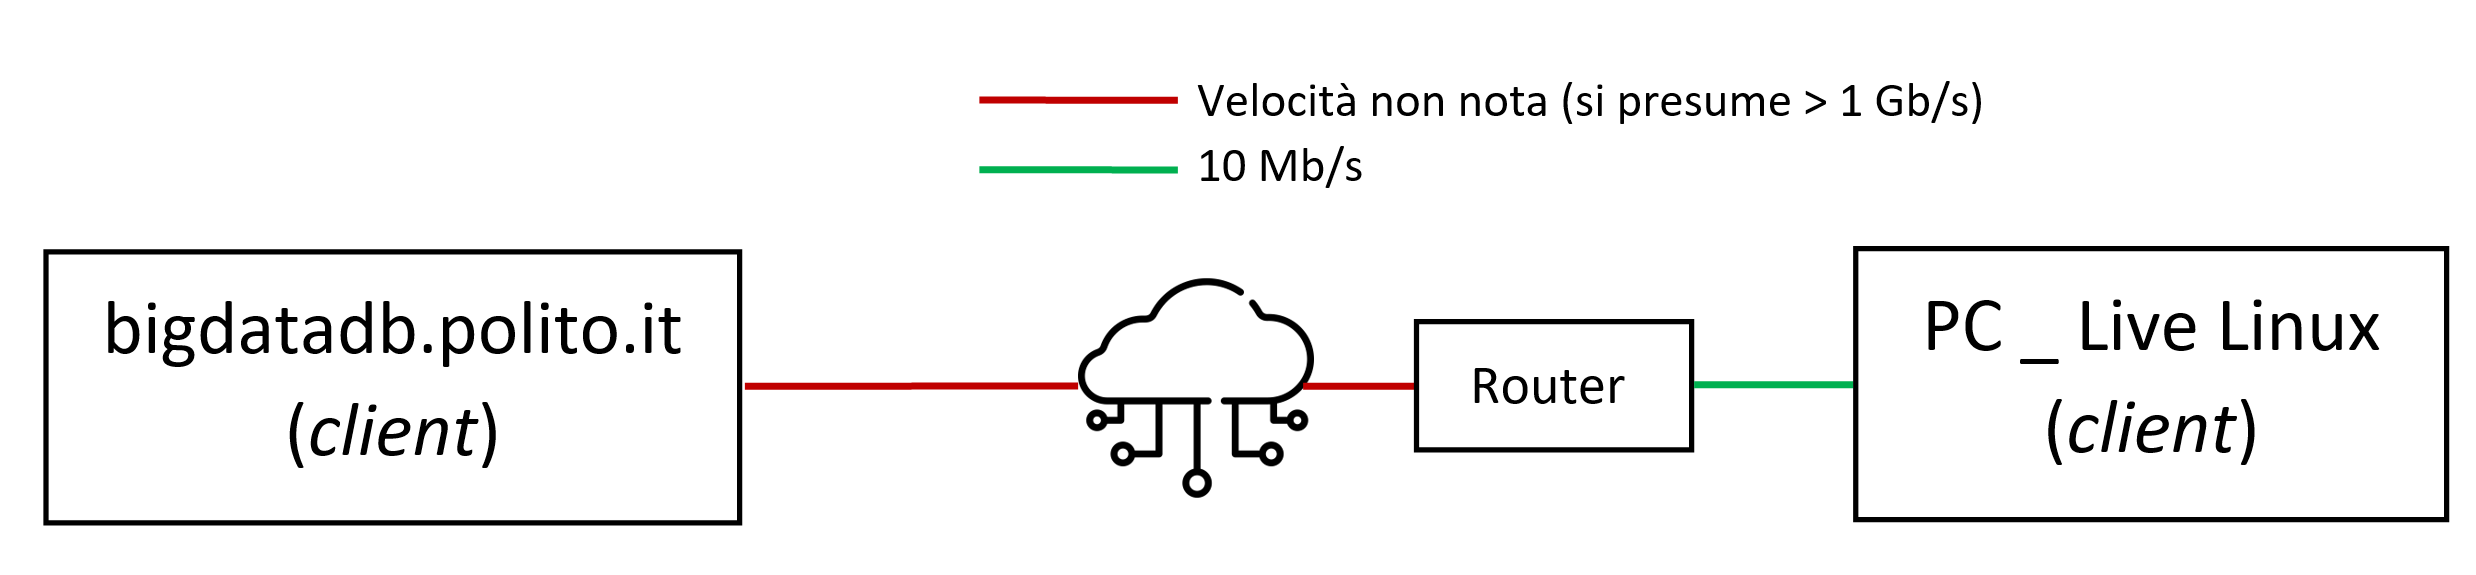
\includegraphics[width=0.6\linewidth]{conf_internet.png}
\end{center}
In questo secondo caso in esame si comunica con un server in rete.
Si ipostizza una velocità dopo il default gateway in media maggiore
di 1 Gb/s (il test è effettuato con fibra FTTH). In tal modo il collo 
di bottiglia è rappresentato dalla velocità tra il nostro Pc è l'home router.

\subsection{Test TCP - Singolo flusso, full duplex}
Eseguendo il comando \textit{iperf3 -c bigdatadb.polito.it} si comunica come 
client con il server. L'efficienza attesa è la stessa calcolata in (4) e 
non ci si aspetta congestione di rete.

\end{document}